\begin{figure}[h!]
    \centering
    \caption{US minimum wage levels by jurisdiction}
    \label{fig:mw_US}

    \begin{subfigure}{.7\textwidth}
        \caption{State level}
        \includegraphics[width = \textwidth]
            {mw_US/output/state_mw_levels.eps}
    \end{subfigure}\\
    \begin{subfigure}{.7\textwidth}
        \caption{Sub-state level}
        \includegraphics[width = \textwidth]
            {mw_US/output/local_mw_levels.eps}
    \end{subfigure}

    \begin{minipage}{.95\textwidth} \footnotesize
        \vspace{3mm}
        Notes:
        Data are from the minimum wage panel described in 
        Section \ref{sec:mw_construction}.
        The plots show the minimum wage levels in the different jurisdictions 
        from January 2010 to December 2019.
        Panel (a) reports the state level policies.
        Panel (b) reports the sub-state level policies.
    \end{minipage}
\end{figure}
